\section{Method}
\label{sec:method}

JPathGene comprises three stages (Fig.~2): modality-specific encoders
and EMA latent targets, bidirectional diffusion-JEPA for cross-modal
latent prediction, and CoRE-Fusion for uncertainty-guided residual
fusion. An optional InfoNCE objective aligns paired image and gene
latents. For each patient, $x_{\mathrm{img}}\in\mathbb{R}^{D}$ denotes
the pre-extracted histopathology feature vector, and
$x_{\mathrm{gene}}\in\mathbb{R}^{G}$ denotes the preprocessed genetic
feature vector.

\begin{figure}[t]
    \centering
    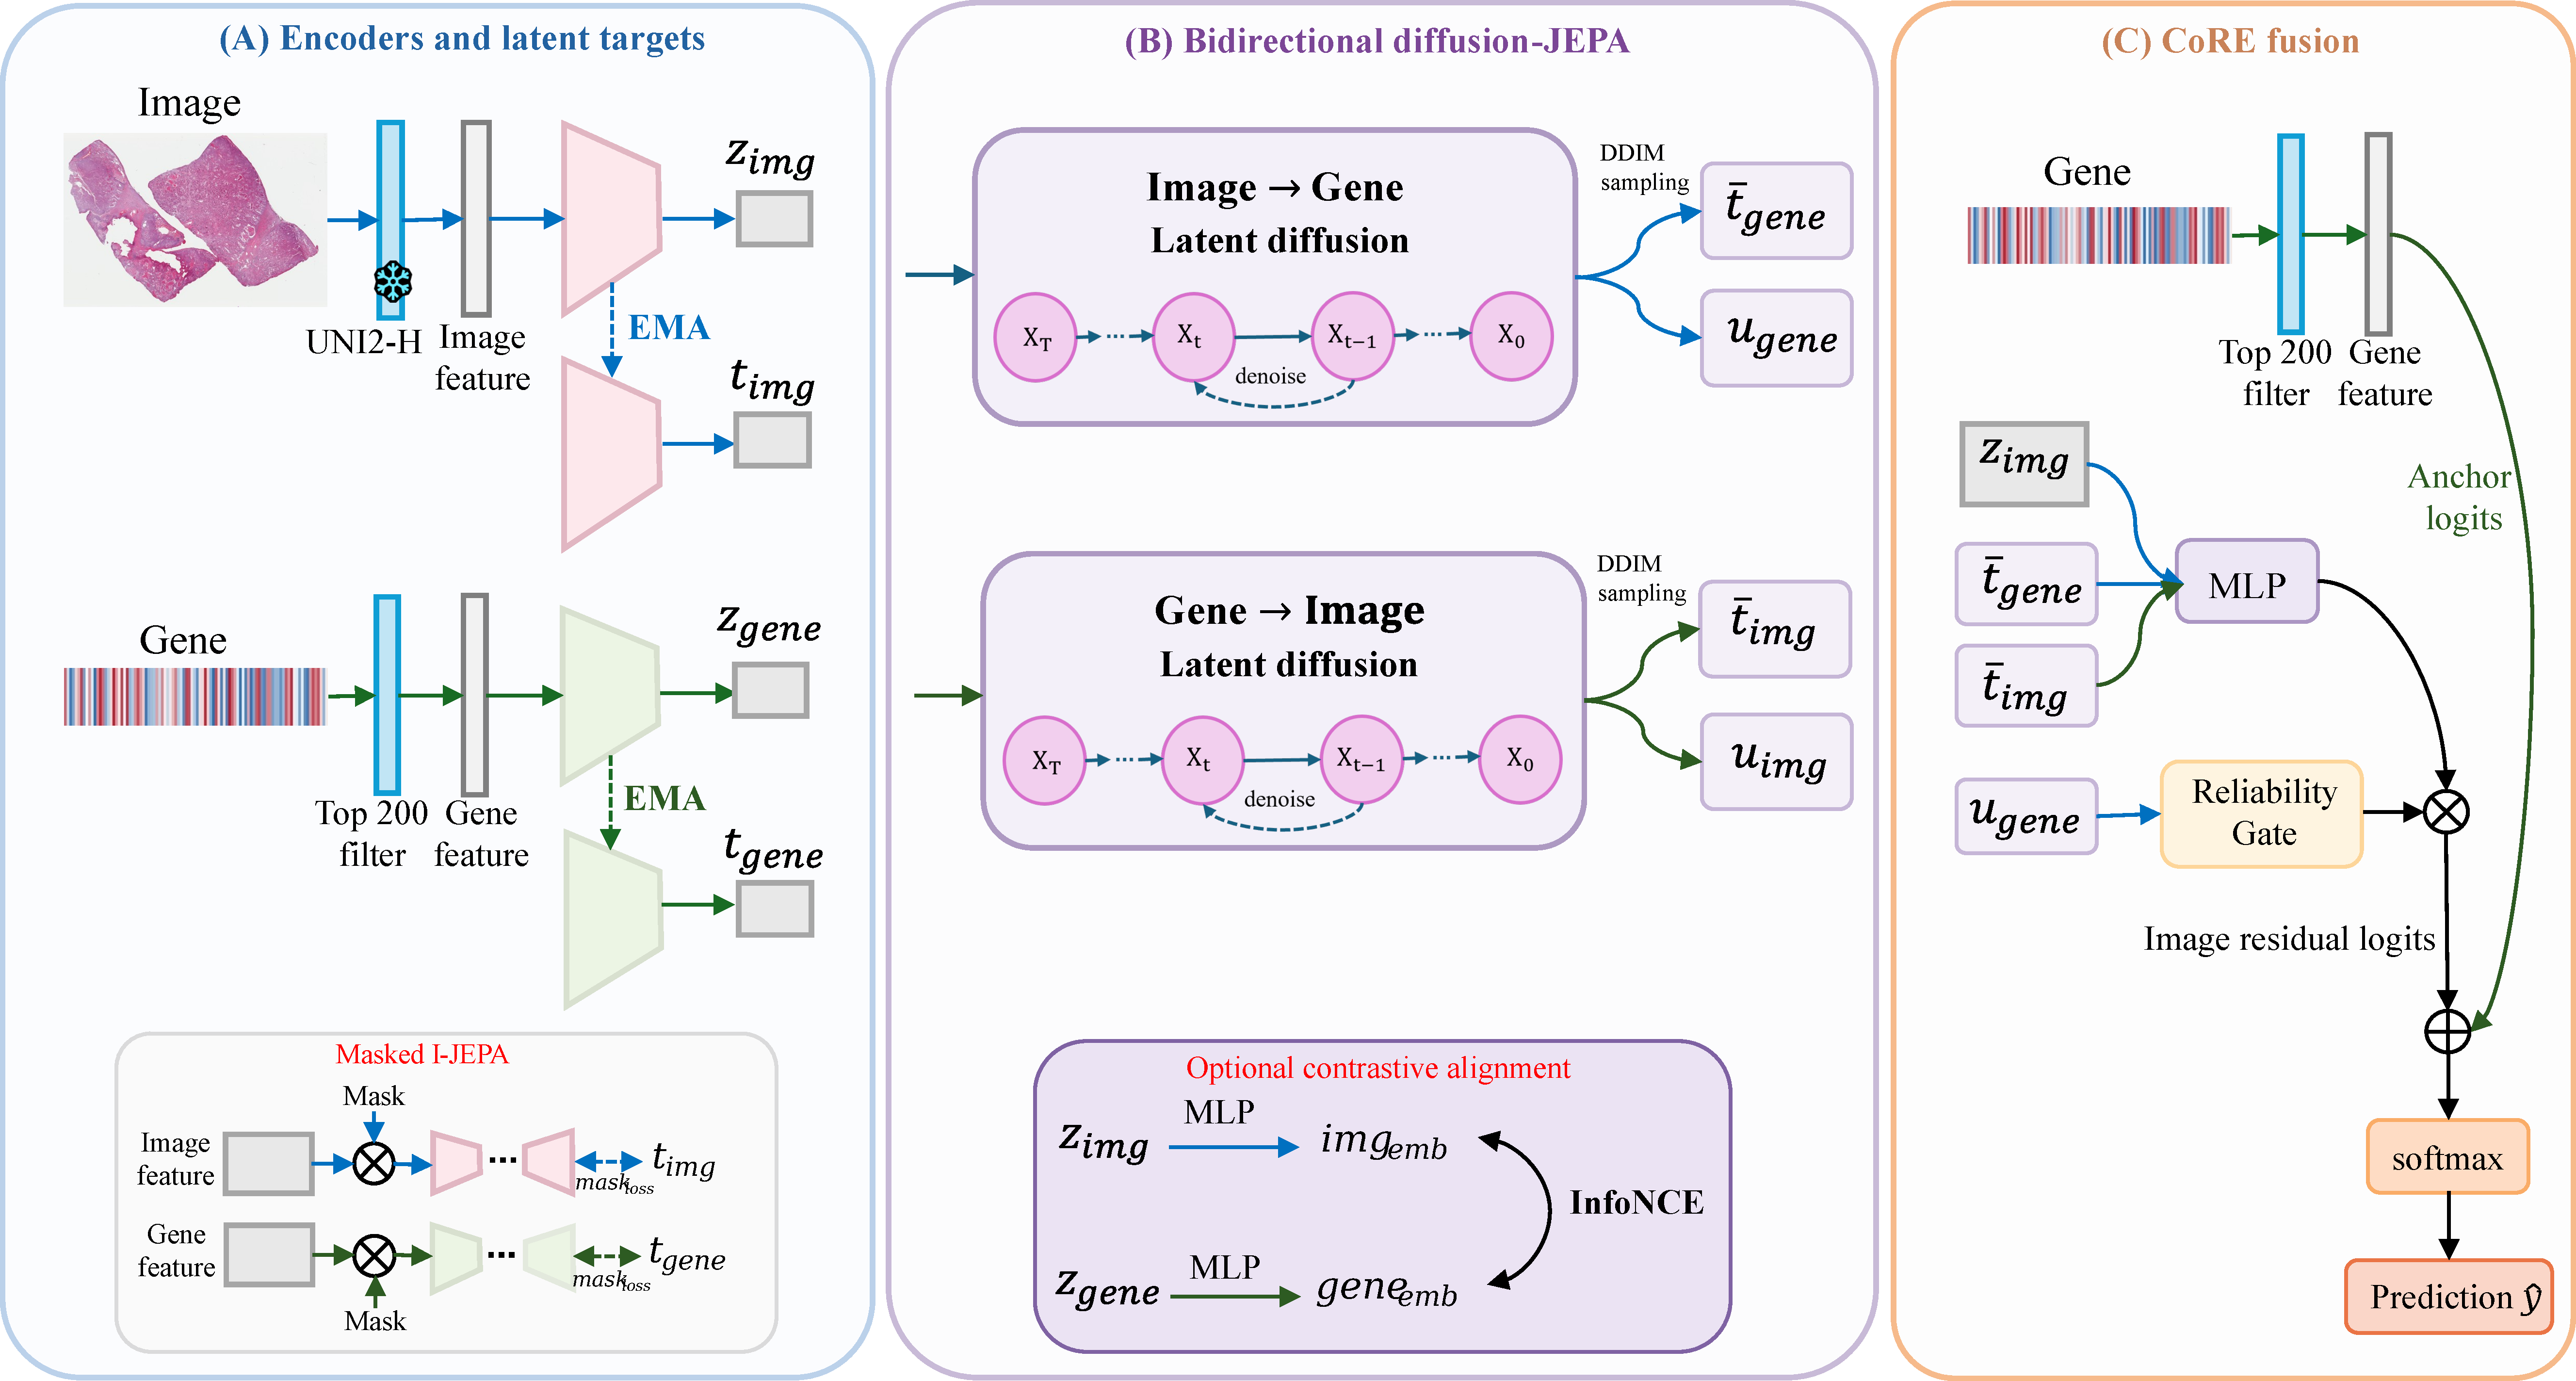
\includegraphics[width=0.95\linewidth]{figures/fig2.pdf}
    \caption{Overview of JPathGene.
(A) Online encoders and EMA teachers produce modality-specific latents and targets.
(B) Bidirectional diffusion-JEPA estimates cross-modal latent means and uncertainties.
(C) CoRE-Fusion uses uncertainty to gate an image residual over genomic anchor logits.}
    \label{fig:architecture}
\end{figure}

\subsection{Encoders and latent targets}
Figure~2A summarizes the online encoders, EMA teachers, and auxiliary masked I-JEPA objective. JPathGene uses pre-extracted histopathology features from a frozen UNI2-h encoder \cite{chen2024uni} and the highest-variance RNA-seq genes. Online encoders $f_{\mathrm{img}}$ and $f_{\mathrm{gene}}$ map them to shared $d$-dimensional latents $\mathbf{z}_{\mathrm{img}}$ and $\mathbf{z}_{\mathrm{gene}}$, using an MLP with optional attention-MIL pooling \cite{ilse2018attention} for images and an MLP or TabTransformer-style tokenizer \cite{huang2020tabtransformer,gorishniy2021ftt} for genes. EMA teachers, updated with momentum $m$, provide stop-gradient targets to prevent collapse. The gene target $t_{\mathrm{gene}}$ is an EMA latent, train-only PCA representation, or pathway-score vector \cite{subramanian2005gsea,liberzon2015hallmark}, while $t_{\mathrm{img}}$ is the image EMA latent. Thus, the model predicts compact latent targets rather than reconstructing raw gene-expression values.

\subsection{Cross-modal diffusion-JEPA}
\label{sec:diffusion}
Figure~2B summarizes bidirectional latent diffusion and DDIM sampling. Deterministic JEPA predicts a single target, but because one histologic phenotype can correspond to multiple genetic programs, we instead model $p(t_{\mathrm{gene}}\mid z_{img})$ and $p(t_{\mathrm{img}}\mid z_{gene})$ with a FiLM-conditioned \cite{perez2018film} latent-diffusion denoiser $\epsilon_\theta$ under a cosine noise schedule $\bar\alpha_\tau$ \cite{ho2020ddpm,nichol2021improved,song2021score}. Because the downstream classifier primarily uses posterior means,
diffusion is not expected to improve point prediction by itself.
Its main role is to represent a conditional latent distribution and
provide patient-specific uncertainty through repeated sampling.

Training follows the standard noise-prediction objective. At a random timestep
$\tau$, a target latent $t$ is perturbed as
$t^{(\tau)}=\sqrt{\bar\alpha_\tau}t+
\sqrt{1-\bar\alpha_\tau}\epsilon$, and $\epsilon_\theta$ predicts the added
noise $\epsilon$ conditioned on the source latent. The same predictor also supports the within-modality masked I-JEPA task \cite{assran2023ijepa}, where the context is a $\rho$-masked view, with deterministic JEPA as the single-step special case (Algorithm~\ref{alg:step}). During both training and inference, $N=8$ DDIM samples \cite{song2021ddim} conditioned on $\zimg$ estimate the posterior mean $\bar t_{\mathrm{gene}}$ and patient-specific uncertainty $u_{\mathrm{gene}}=\tfrac{1}{d}\sum_{j=1}^{d}\operatorname{std}_{n}[\hat t_{\mathrm{gene},j}^{n}]$; the uncertainty feeds the CoRE gate below, so sampling is part of each training step. Here, $t_{\mathrm{gene}}\in\mathbb{R}^{d}$ denotes the full genetic target latent, and $\hat t_{\mathrm{gene},j}^{n}$ denotes the $j$-th component of its $n$-th sampled prediction; $\bar t_{\mathrm{img}}$ and $u_{\mathrm{img}}$ are defined analogously.

\begin{algorithm}[t]
\caption{JPathGene training}
\label{alg:step}
\begin{algorithmic}[1]
\Require paired data $\mathcal{D}\!=\!\{(x^{\mathrm{img}}_i,x^{\mathrm{gene}}_i,y_i)\}$; online encoders $f_{\mathrm{img}},f_{\mathrm{gene}}$, denoiser $\epsilon_\theta$, projection heads $h_{\mathrm{img}},h_{\mathrm{gene}}$, fusion heads $g_{\mathrm{anchor}},g_{\mathrm{img}}$, gate $(w,b)$; EMA decay $m$; loss weights $\lambda_k$
\For{each training epoch}
\For{each minibatch $(x^{\mathrm{img}},x^{\mathrm{gene}},y)\in\mathcal{D}$}
\State $\zimg\!\gets\!f_{\mathrm{img}}(x^{\mathrm{img}})$, $\zgene\!\gets\!f_{\mathrm{gene}}(x^{\mathrm{gene}})$ \Comment{online (student) latents}
\State $t_{\mathrm{img}},t_{\mathrm{gene}}\!\gets\!\textsc{StopGrad}$ EMA teachers \Comment{or PCA/pathway $t_{\mathrm{gene}}$}
\State draw $\tau\!\sim\!\mathcal{U}\{1,T\}$, $\epsilon\!\sim\!\mathcal{N}(0,I)$; $\;t^{(\tau)}\!\gets\!\sqrt{\bar\alpha_\tau}\,t+\sqrt{1-\bar\alpha_\tau}\,\epsilon$
\State $\mathcal{L}_{\mathrm{i\to g}}\!\gets\!\|\epsilon-\epsilon_\theta(t^{(\tau)}_{\mathrm{gene}},\tau,\zimg)\|_2^2$; symmetric $\mathcal{L}_{\mathrm{g\to i}}$ \Comment{cross-modal JEPA}
\State $\mathcal{L}^{\mathrm{mask}}_{\mathrm{gene}}\!\gets\!\|\epsilon-\epsilon_\theta(t^{(\tau)}_{\mathrm{gene}},\tau,\zgene^{\mathrm{ctx}})\|_2^2$; symmetric $\mathcal{L}^{\mathrm{mask}}_{\mathrm{img}}$ \Comment{$\rho$-masked, same $\epsilon_\theta$}
\State $\mathcal{L}_{\mathrm{align}}\!\gets\!\textsc{InfoNCE}(h_{\mathrm{img}}(\zimg),h_{\mathrm{gene}}(\zgene))$ \Comment{optional}
\State $\bar t_{\mathrm{gene}},\bar t_{\mathrm{img}},u_{\mathrm{gene}}\!\gets\!\textsc{DDIM-Sample}(\epsilon_\theta,N)$ \Comment{mean + uncertainty, no grad}
\State $\alpha\!\gets\!\sigma\!\big(w(-u_{\mathrm{gene}})+b\big)$; $\;\hat y\!\gets\!g_{\mathrm{anchor}}(x^{\mathrm{gene}})+\alpha\,g_{\mathrm{img}}([\zimg,\bar t_{\mathrm{gene}},\bar t_{\mathrm{img}}])$; $\;\mathcal{L}_{\mathrm{cls}}\!\gets\!\mathrm{CE}(\hat y,y)$ \Comment{CoRE gate}
\State $\mathcal{L}\!\gets\!\textstyle\sum_{k}\lambda_k\mathcal{L}_k$, $k\in\{$i$\to$g, g$\to$i, mask, align, cls$\}$; update online $\Theta$ by $\nabla_\Theta\mathcal{L}$
\State EMA-update teachers: $\theta^{-}\!\gets\!m\,\theta^{-}+(1-m)\,\theta$
\EndFor
\EndFor
\end{algorithmic}
\end{algorithm}

\subsection{CoRE: complementary residual experts}
\label{sec:core}
For molecular endpoints, genomic features are often more predictive than histology, so naive multimodal fusion may underperform a gene-only model. \textbf{CoRE-Fusion} therefore retains a genomic anchor $g_{\mathrm{anchor}}(x_{\mathrm{gene}})$ and adds an uncertainty-gated image residual (Fig.~\ref{fig:architecture}):
\begin{equation}
\begin{aligned}
\hat{y}
&= g_{\mathrm{anchor}}(x_{\mathrm{gene}})
 + \alpha\, g_{\mathrm{img}}
 \bigl([z_{\mathrm{img}},\bar{t}_{\mathrm{gene}},
 \bar{t}_{\mathrm{img}}]\bigr), \\
\alpha
&= \sigma(-w u_{\mathrm{gene}}+b)\in(0,1).
\end{aligned}
\end{equation}
where $\sigma$ is the logistic function and $b$ and $w$ are learned scalars.
Both $g_{\mathrm{anchor}}$ and $g_{\mathrm{img}}$ output classification logits,
which are summed. The gate maps cross-modal uncertainty to a patient-specific
image-residual weight. The reported models use the soft gate, which continuously adjusts
rather than hard-thresholds the image contribution. The total
objective combines cross-modal prediction, masked prediction,
latent alignment, and classification losses, with
$\lambda_{i\rightarrow g}=\lambda_{g\rightarrow i}=\lambda_{\mathrm{cls}}=1$,
$\lambda_{\mathrm{mask}}=0.5$, and $\lambda_{\mathrm{align}}=0.1$,
and is optimized using AdamW.